% Local Agentic RAG for PDFs: final competition report (pdfLaTeX).
% Started from ../main.tex (the progress report); that file and its PDF are unchanged.
% Build: ./build.sh   (pdfLaTeX in the texlive/texlive Docker image, repository root mounted for the figures)
% Every number below is measured and labelled with its run. docs/RESULTS.md, docs/SCALE.md and docs/STATUS.md
% list where each one comes from. Dev set = the 61 English + 20 multilingual questions used during development;
% held-out = documents whose questions were written independently and used exactly once.
\documentclass[10pt,a4paper]{article}

\usepackage[T1]{fontenc}
\usepackage[default,semibold]{sourcesans}
\usepackage[a4paper,top=15mm,bottom=17mm,left=17mm,right=17mm]{geometry}
\usepackage{microtype}
\usepackage{xcolor}
\usepackage{graphicx}
\graphicspath{{figures/}{../docs/img/}}
\usepackage{tikz}
\usetikzlibrary{arrows.meta,positioning,calc}
\usepackage{pgfplots}
\pgfplotsset{compat=1.18}
\usepackage[most]{tcolorbox}
\usepackage{booktabs}
\usepackage{tabularx}
\usepackage{array}
\usepackage{enumitem}
\usepackage{titlesec}
\usepackage{fontawesome5}
\usepackage{multicol}
\usepackage{fancyhdr}
\usepackage[hidelinks]{hyperref}
\hypersetup{pdftitle={Local Agentic RAG for PDFs: final report},pdfauthor={Satyam Kumar Pandey}}

% ---------------------------------------------------------------- colours
\definecolor{navy}{HTML}{14213D}
\definecolor{ink}{HTML}{1F2937}
\definecolor{muted}{HTML}{5B6573}
\definecolor{amber}{HTML}{C2620F}
\definecolor{cyan}{HTML}{2F8FB8}
\definecolor{teal}{HTML}{2A9D8F}
\definecolor{paper}{HTML}{F3F6FA}
\definecolor{rule}{HTML}{D5DCE6}
\definecolor{good}{HTML}{2E8B57}
\definecolor{warn}{HTML}{B4560F}

\color{ink}
\setlength{\parindent}{0pt}
\setlength{\parskip}{4pt}
\linespread{1.06}

\pagestyle{fancy}
\fancyhf{}
\renewcommand{\headrulewidth}{0pt}
\fancyfoot[L]{\color{muted}\fontsize{7.5}{9}\selectfont Local Agentic RAG for PDFs \enspace·\enspace final report}
\fancyfoot[R]{\color{muted}\fontsize{7.5}{9}\selectfont\thepage}

% ---------------------------------------------------------------- headings
\titleformat{\section}{\color{navy}\fontsize{13.5}{16}\selectfont\bfseries}
  {\color{amber}\thesection\hspace{6pt}}{0pt}{}
\titlespacing*{\section}{0pt}{10pt}{4pt}
\titleformat{\subsection}{\color{navy}\fontsize{10.5}{13}\selectfont\bfseries}{}{0pt}{}
\titlespacing*{\subsection}{0pt}{6pt}{2pt}

\setlist{nosep,leftmargin=12pt,topsep=2pt,itemsep=1.5pt}
\setlist[itemize]{label={\color{amber}\small$\bullet$}}

% ---------------------------------------------------------------- helpers
\newcommand{\kicker}[1]{{\color{amber}\fontsize{8}{10}\selectfont\bfseries\MakeUppercase{#1}}}
\newcommand{\note}[1]{{\raggedright\color{muted}\fontsize{8.3}{10}\selectfont #1\par}}

% metric card: value, label, footnote
\newcommand{\metric}[3]{%
  \begin{tcolorbox}[enhanced,colback=paper,colframe=paper,arc=3pt,
      left=7pt,right=5pt,top=5pt,bottom=5pt,height=27mm,valign=top,
      borderline west={2.5pt}{0pt}{amber}]\raggedright
    {\color{navy}\fontsize{19}{21}\selectfont\bfseries #1}\par\vspace{1pt}
    {\fontsize{8.6}{10.2}\selectfont\bfseries #2}\par\vspace{1pt}
    {\color{muted}\fontsize{7.4}{9}\selectfont #3}
  \end{tcolorbox}}

\newtcolorbox{panel}[1][]{enhanced,colback=paper,colframe=paper,arc=3pt,
  left=8pt,right=8pt,top=6pt,bottom=6pt,#1}

\newcommand{\done}{{\color{good}\faCheckCircle}}

\begin{document}

% =====================================================================
% Cover, results at a glance, abstract
% =====================================================================
\thispagestyle{empty}
\begin{tikzpicture}[remember picture,overlay]
  \node[anchor=north,inner sep=0] at (current page.north)
    {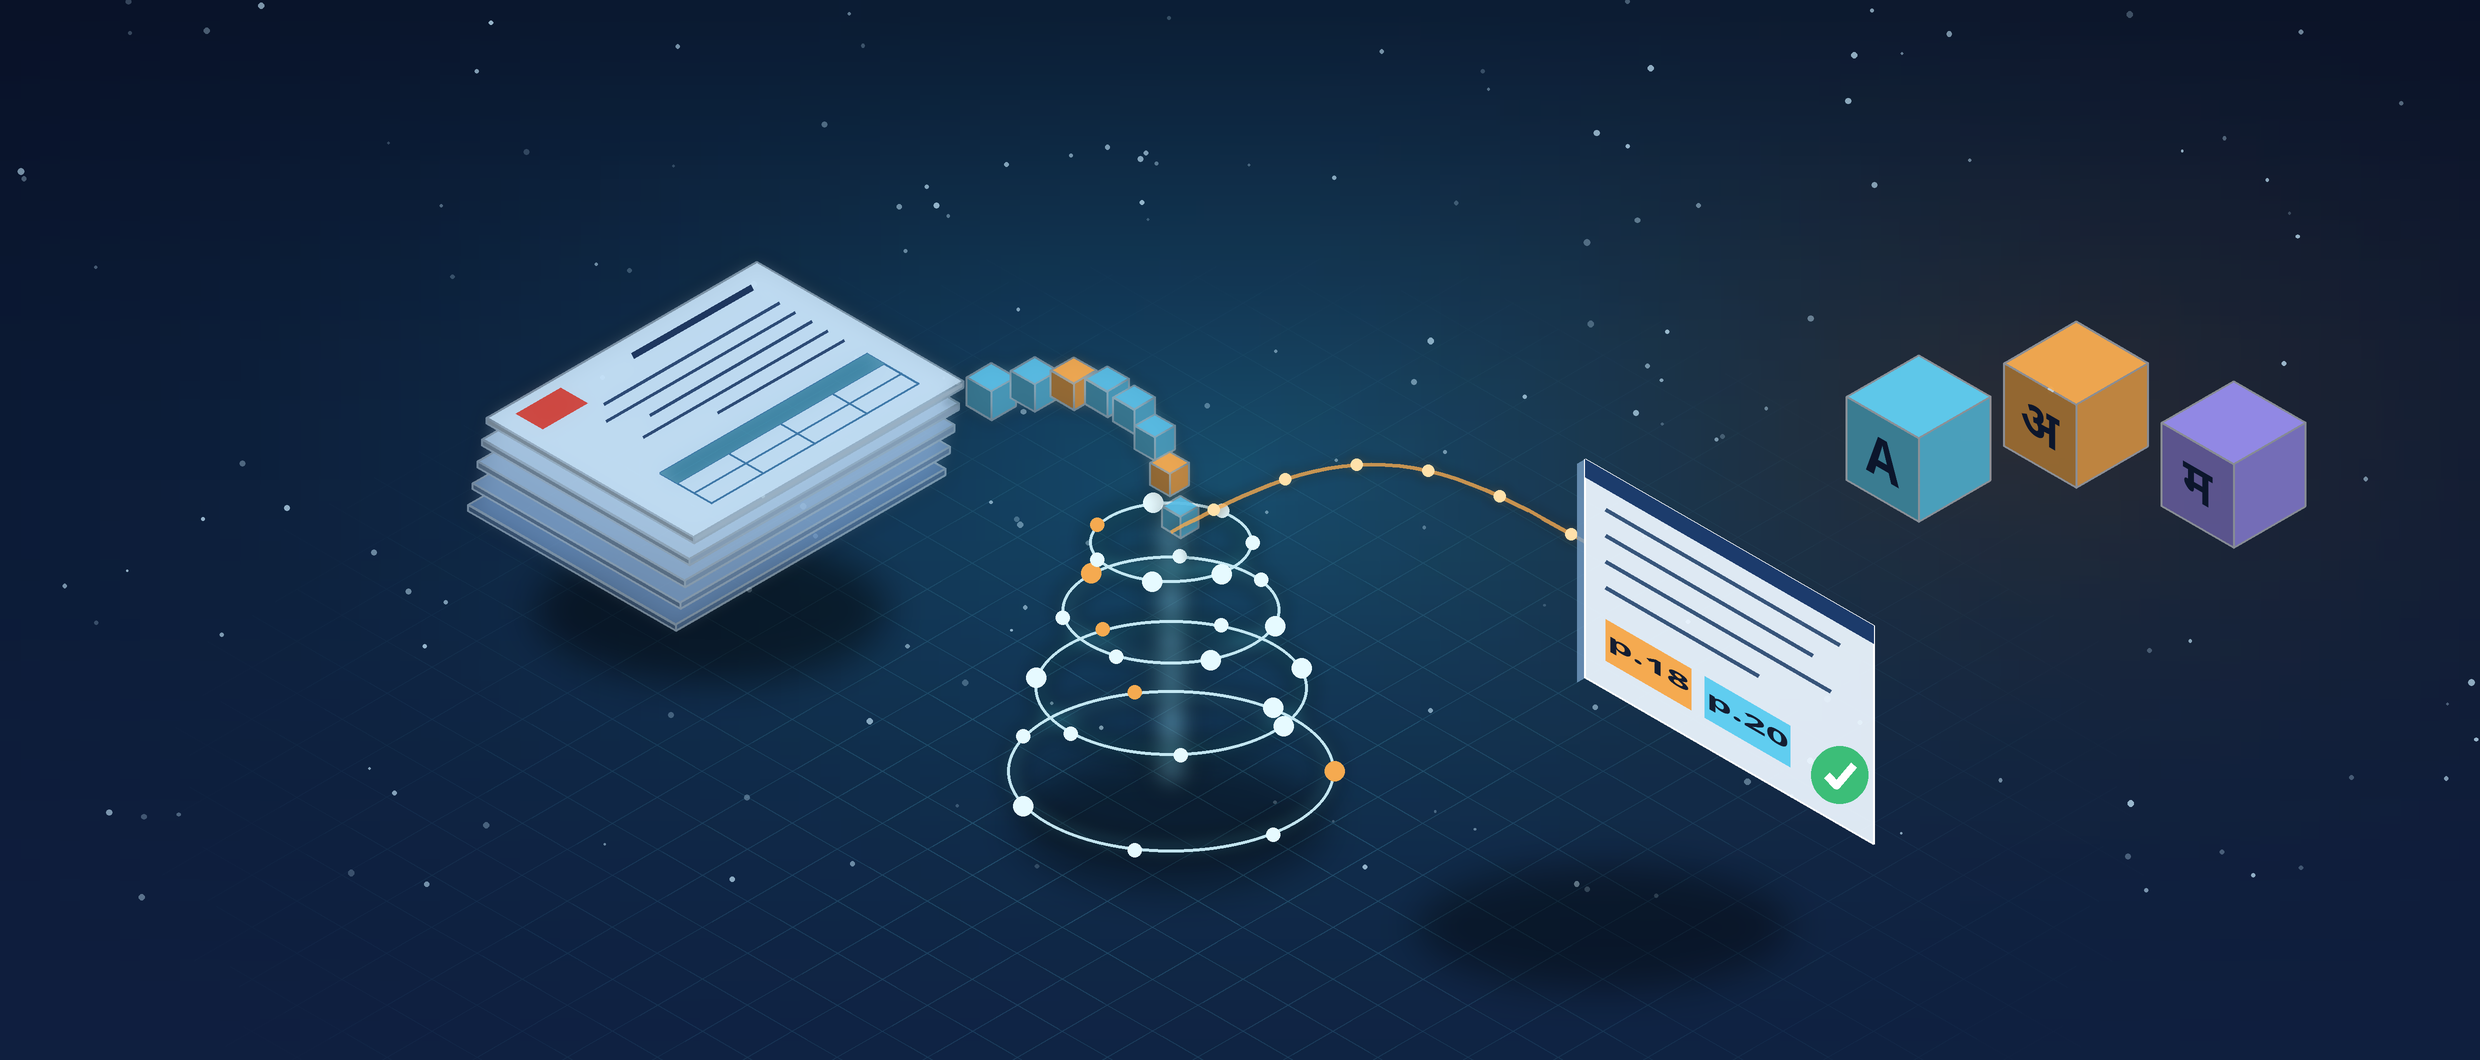
\includegraphics[width=\paperwidth]{cover.png}};
  \node[anchor=north west,text=white,font=\fontsize{8}{10}\selectfont\bfseries]
    at ([xshift=17mm,yshift=-11mm]current page.north west)
    {\MakeUppercase{UTMT Local PDF Chatbot Competition \enspace·\enspace final report}};
\end{tikzpicture}

\vspace*{78mm}

{\color{navy}\fontsize{25}{29}\selectfont\bfseries Local Agentic RAG for PDFs}\par
\vspace{3pt}
{\color{muted}\fontsize{12}{15}\selectfont Cited answers from PDFs of up to 10,000 pages, tested in 22 languages from Sanskrit and Bhojpuri to Urdu, Telugu and Chinese,
using only open-weight models on one T4 GPU}\par
\vspace{8pt}
\begin{tabularx}{\textwidth}{@{}X r@{}}
  {\fontsize{9.5}{12}\selectfont\bfseries Satyam Kumar Pandey}\enspace
  {\color{muted}\fontsize{9}{12}\selectfont\enspace Team PageProof}
  &
  \tcbox[on line,colback=navy,colframe=navy,arc=8pt,left=6pt,right=6pt,top=2pt,bottom=2pt]
    {\color{white}\fontsize{8.5}{10}\selectfont\bfseries Final report}
\end{tabularx}

\vspace{6pt}
\kicker{Results at a glance (Kaggle T4 runs)}\par\vspace{3pt}
\begin{tcbraster}[raster columns=4,raster equal height,raster column skip=6pt,raster row skip=6pt,raster before skip=0pt,raster after skip=0pt]
  \metric{84.6\%}{answer accuracy, dev set}{44/52 answerable English questions; 95\% interval 73.1--94.2\%}
  \metric{1/52}{same model, no documents}{the answers come from retrieval, not from the model's memory}
  \metric{43/57}{held-out documents}{GAO 15/18, US Code Title 21 19/25, Hindi audit 9/14; each used once}
  \metric{9/9}{unanswerable refused}{English dev questions with no answer in the document}
  \metric{94.2\%}{page recall@5}{evidence page in the top 5; 73.1\% for the starting code}
  \metric{85/111}{22 languages, dev set}{117/122 answered in the right script; 33/44 and 18/20 on 16 unseen documents}
  \metric{36.9 min}{for 10,000 pages}{table-heavy PDF on a T4, with crash recovery}
  \metric{8.9 GB}{GPU memory in use}{of 15 GB, with all three models loaded}
\end{tcbraster}

\vspace{4pt}
\begin{panel}
\fontsize{9.2}{11.6}\selectfont
\textbf{Summary.} Local Agentic RAG answers questions about any uploaded PDF and cites the pages it used.
It runs only open-weight models on a single free T4 GPU, with no outside AI service and no API key. Ingestion reads PDFs in
reading order, rebuilds tables row by row, OCRs scanned pages and indexes them in checkpointed batches, so a 10,000-page PDF is processed with crash recovery and can be
queried while it is still being read. Each question runs a hybrid search (BGE-M3 meaning search and BM25 keyword search, fused by rank), a multilingual reranker keeps six passages,
and Qwen2.5-7B writes an answer that must cite them. A verifier checks every claim. Only when the answer is refused or unsupported does the agent plan sub-questions, search again and rewrite,
and a Python calculator does the arithmetic. Every design choice, including the choice of answer model among five candidates, was measured on a T4. A web app streams answers, opens the
cited page with the passage highlighted, and serves several users through a visible queue.
\end{panel}

\section{The problem and the goal}
Long PDFs such as statutes, budget documents, statistical abstracts and audit reports are hard to search.
Hosted chatbots can answer questions about them, but they cost money, send the document to a third party,
and often answer confidently when the PDF does not say. We build for people who cannot or should not upload such files:
law students and small firms working with statutes and contracts, government and NGO analysts in India with
budget books, statistical abstracts and scanned Hindi or Marathi circulars, researchers, and compliance teams.
The goal is a local tool that answers questions about \emph{any} uploaded PDF, from a few pages to 10,000 pages,
under four constraints:
\begin{itemize}
  \item \textbf{Local only.} Open-weight models and no API keys, so the document never leaves the machine.
  \item \textbf{Free hardware.} One T4 as on free Colab: 15 GB GPU memory, 12.7 GB host RAM, 2 vCPUs.
  \item \textbf{Grounded.} Every answer cites the pages it used, or says the document does not contain the answer.
  \item \textbf{Multilingual.} Questions and documents may be in different languages, and scanned pages must work.
\end{itemize}
We started from the reference notebook and an early codebase that had only a non-agentic baseline
(MiniLM search, no tables, no OCR, English only). We rebuilt ingestion, retrieval and the agent, measured
every change on a fixed benchmark, scaled ingestion to 10,000 pages, added a multi-user web app, and finally checked
the system on documents it had never seen.

% =====================================================================
\section{Architecture: the end-to-end flow}
The system has two paths. \textbf{Ingestion} runs once per PDF and is cached by file hash.
\textbf{Answering} runs per question. One pass that retrieves, answers and verifies handles most questions;
the agent loop starts only when that pass refuses or the verifier finds an unsupported claim.
Figure 1 follows one real question from a recording session on a free Colab T4.

\begin{center}
\begin{tcolorbox}[enhanced,colback=white,colframe=rule,boxrule=0.6pt,arc=3pt,left=0pt,right=0pt,top=0pt,bottom=0pt,width=0.97\textwidth]
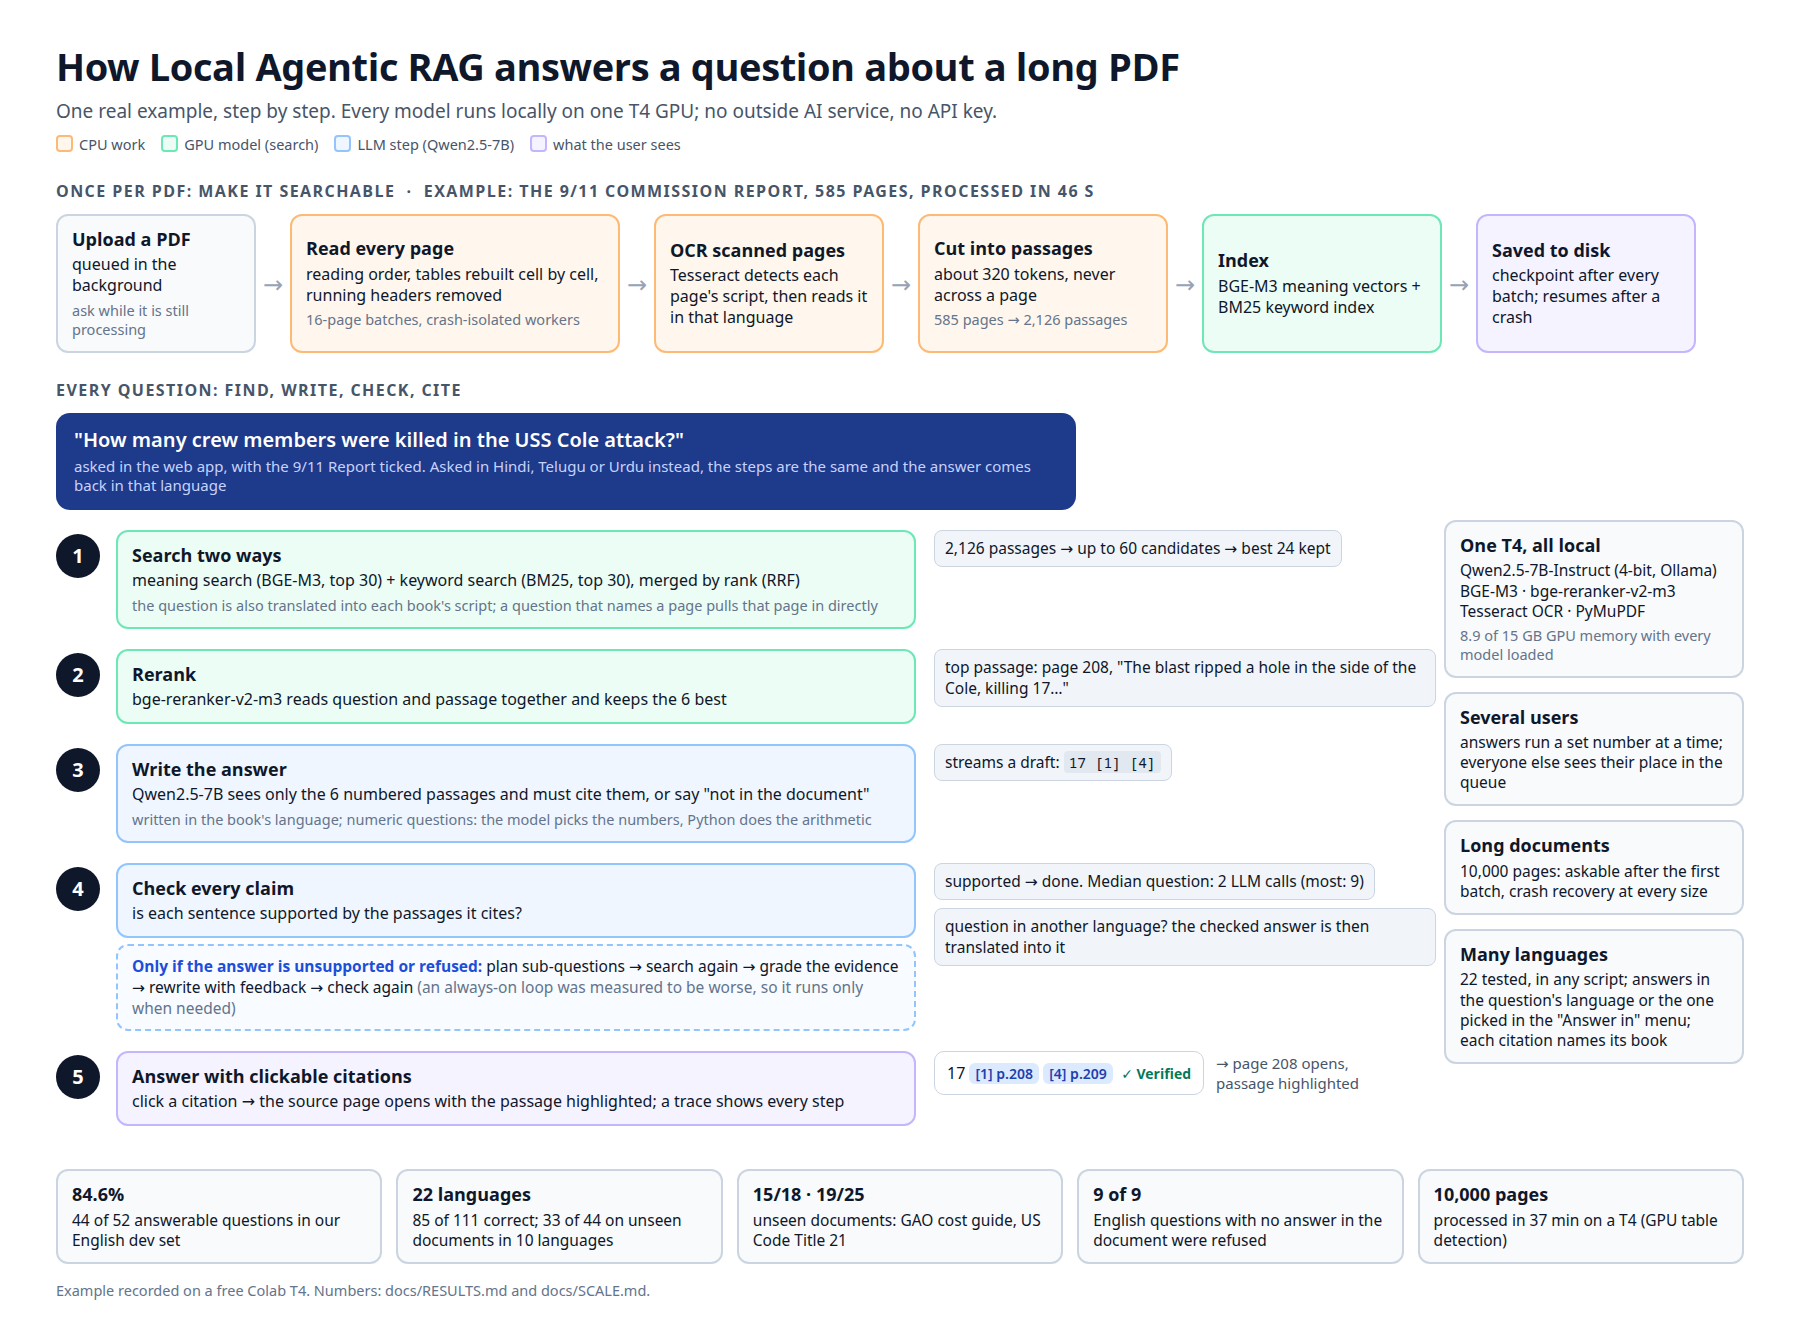
\includegraphics[width=\linewidth]{workflow.png}
\end{tcolorbox}
\vspace{2pt}\note{\textbf{Figure 1.} The workflow on one example: the 9/11 Commission Report (585 pages, 2,126 passages, processed in 46\,s) and the question
``How many crew members were killed in the USS Cole attack?''. The answer, 17, cites pages 208 and 209 and is marked verified.}
\end{center}

\vspace{-6pt}
\textbf{Per question.} (1) If there is chat history, a follow-up is rewritten as a standalone question; if the question's language differs from the document's,
one LLM call translates it, and passages are ranked by the better of the original and the translation; a page named in the question (``page 4,512'') pulls that page's
passages into the pool. (2) BGE-M3 dense search and BM25 keyword search each return 30 candidates, reciprocal rank fusion keeps 24, and the cross-encoder reranker keeps 6.
(3) For a question that needs arithmetic, the LLM picks a structured operation and copies the operands with citations, each operand is checked against the cited row and column,
and Python computes the result. (4) Qwen2.5-7B answers from the six numbered passages, citing each claim as [n], or replies that the document does not contain the answer.
(5) The verifier checks every claim against the passages it cites. If the answer is supported, it is returned. Otherwise the agent plans sub-questions, retrieves again
(still ranked by the user's question; each sub-question only adds its best passage), drops passages that both the grader and the reranker reject, and rewrites with feedback.
In the regression run (run 3) the median question used \textbf{2 LLM calls} and the most was 9. Structured steps use JSON-schema constrained output, and every step falls back
to the simpler path if its output is invalid (in run 8 no model produced an invalid JSON step).

% =====================================================================
\section{Ingesting long PDFs}
The first design parsed the whole PDF in memory and saved the index at the end. That works for 60 pages and fails at 10,000:
memory grows with the document, one malformed page can crash the process, and a disconnect after an hour loses everything.
Ingestion is now a two-pass stream with checkpoints:
\begin{itemize}
  \item \textbf{Pass 1, read (CPU, parallel).} Worker processes parse 16-page batches: column-aware reading order, ruled tables to Markdown, whitespace-aligned tables
        rebuilt from word coordinates as labelled rows (\texttt{label | 2025 Q2 = 3.8}), and OCR for image-only or garbled pages (Tesseract at 300 dpi, \texttt{eng+hin+mar}).
        Pass 1 also counts the document-wide facts that pass 2 needs: margin lines that repeat on 40\% of pages (running headers) and the body font size (for headings).
  \item \textbf{Pass 2, index (in page order).} Strip running headers and footers, cut passages of at most 320 embedder tokens at headings, paragraphs and sentences
        (never across a page, with a ``title \textgreater{} section'' header), embed 48-page batches on the GPU, and write float16 vectors to disk. The BM25 matrix is built at the end.
  \item \textbf{Crash isolation.} A page that crashes the PDF library or exceeds its time budget kills only its worker: that page becomes an empty page with a warning,
        the worker restarts and the batch continues.
  \item \textbf{Resumable.} Each pass appends, fsyncs, then atomically replaces a checkpoint file. A crash, a cancelled job or a closed notebook resumes from the last checkpoint.
  \item \textbf{Ask while processing.} A document becomes askable at its first pass-2 checkpoint, and answers say which pages they were drawn from
        (``answered from the first $n$ of $N$ pages''). A 1,000-page PDF was askable 206\,s after upload, with 96 pages indexed, and the answer was correct and cited (run 1).
\end{itemize}

% =====================================================================
\section{Retrieval and agent design, and the evidence behind it}
\renewcommand{\arraystretch}{1.2}
{\fontsize{8.4}{10.1}\selectfont
\begin{tabularx}{\textwidth}{@{}>{\raggedright\arraybackslash\bfseries}p{36mm} >{\raggedright\arraybackslash}X >{\raggedright\arraybackslash}p{54mm}@{}}
\toprule
\color{navy}Decision & \color{navy}\textbf{Why} & \color{navy}\textbf{Measured effect} \\ \midrule
Hybrid search + cross-encoder reranker & Dense search finds paraphrases, BM25 finds exact labels and numbers, and the reranker reads question and passage together. & Page recall@5 94.2\% (multilingual default; 96.2\% with English-only models); a basic MiniLM search: 73.1\% \\
Table rebuilding & Statistical tables are aligned with spaces, so plain text extraction scrambles rows and columns. & Table questions rose from 42\% to 83\%, helped by better retrieval and table captions \\
BGE-M3 + multilingual reranker & English-only models miss Hindi and Hinglish wording. & Multilingual set: recall@5 1.00 and MRR 0.97 (English-only models: 0.94 and 0.88), with answer accuracy tied \\
Adaptive agent, not an always-on loop & Our first always-on loop was \emph{worse} than a single pass (23 vs 27 of 38): sub-queries crowded out the real evidence. & The loop runs only when needed, with fewer false refusals at similar accuracy \\
Python calculator + number fixes & The 7B model picked the wrong measure or the wrong table cell, and sometimes subtracted wrong. & Numerical questions 5/6 (2/6 without them); English 84.6\% (76.9\% without them; runs 5--6) \\
Tesseract CLI OCR at 300 dpi & The built-in OCR path lost about 30\% of the Hindi words on scanned pages. & Hindi word recall 0.99 and 1.00 (built-in OCR: 0.70) \\
\bottomrule
\end{tabularx}}

\vspace{4pt}
\begin{minipage}[t]{0.49\textwidth}
\subsection{Retrieval: is the evidence page in the top 5?}
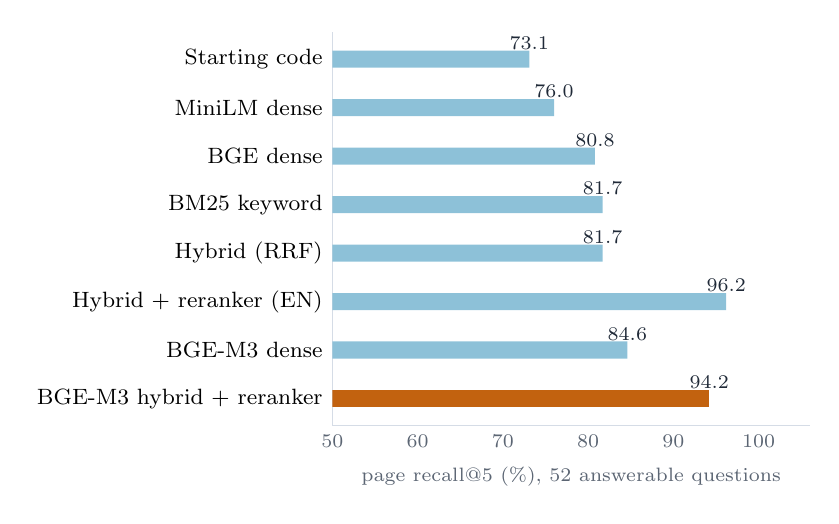
\begin{tikzpicture}
\begin{axis}[
    xbar, scale only axis, width=0.50\linewidth, height=50mm, bar width=6.2pt, bar shift=0pt,
    xmin=50, xmax=106, xtick={50,60,70,80,90,100}, axis x line*=bottom, axis y line*=left,
    xlabel={page recall@5 (\%), 52 answerable questions}, xlabel style={font=\fontsize{7.5}{9}\selectfont,text=muted},
    symbolic y coords={start,minilm,bge,bm25,hybrid,rerank,m3dense,m3rerank},
    ytick={start,minilm,bge,bm25,hybrid,rerank,m3dense,m3rerank}, y dir=reverse,
    yticklabels={Starting code, MiniLM dense, BGE dense, BM25 keyword, Hybrid (RRF), Hybrid + reranker (EN), BGE-M3 dense, BGE-M3 hybrid + reranker},
    yticklabel style={font=\fontsize{7.6}{9}\selectfont,align=right},
    xticklabel style={font=\fontsize{7.5}{9}\selectfont,text=muted},
    nodes near coords, nodes near coords style={font=\fontsize{7.4}{9}\selectfont,text=ink},
    point meta=explicit symbolic, enlarge y limits=0.08,
    axis line style={draw=rule}, major tick length=0pt]
  \addplot[fill=cyan!55,draw=none] coordinates {
    (73.1,start)[73.1] (76.0,minilm)[76.0] (80.8,bge)[80.8] (81.7,bm25)[81.7]
    (81.7,hybrid)[81.7] (96.2,rerank)[96.2] (84.6,m3dense)[84.6]};
  \addplot[fill=amber,draw=none] coordinates {(94.2,m3rerank)[94.2]};
\end{axis}
\end{tikzpicture}\par
\note{Orange is the default (multilingual). The reranker is the largest single gain.
The multilingual default is one question below the English-only reranker here and ranks best at top-1 (68.3\%).}
\end{minipage}\hfill
\begin{minipage}[t]{0.47\textwidth}
\subsection{Answers end to end (Kaggle T4)}
\renewcommand{\arraystretch}{1.22}
{\fontsize{8.4}{10.2}\selectfont
\begin{tabularx}{\linewidth}{@{}X r r r@{}}
\toprule
 & \textbf{Baseline} & \textbf{Single pass} & \textbf{Agent} \\ \midrule
Answer accuracy      & 50.0\% & 71.2\% & \textbf{76.9\%} \\
Fact recall          & 53.2\% & 74.7\% & 80.1\% \\
False refusals       & 26.9\% & 3.8\%  & 1.9\% \\
Unanswerable refused & 9/9    & 9/9    & 9/9 \\
Citation precision   & 70.6\% & 73.7\% & 78.4\% \\
Latency, median      & 2.7 s  & 3.2 s  & 6.6 s \\
\bottomrule
\end{tabularx}}
\note{Same 61 English dev questions and LLM in every column. ``Baseline'' is the starting design (MiniLM search, single pass).
``Agent'' is the default (adaptive loop + calculator). 95\% intervals are about $\pm$12 points, so the last two columns differ within noise.
The number fixes then raised the agent to 84.6\% (next table).}
\end{minipage}

\vspace{4pt}
\begin{minipage}[t]{0.49\textwidth}
\subsection{Number fixes (dev set, runs 5 and 6)}
\renewcommand{\arraystretch}{1.2}
{\fontsize{8.4}{10.2}\selectfont
\begin{tabularx}{\linewidth}{@{}X r r@{}}
\toprule
English dev set & Without the fixes & \textbf{With them (default)} \\ \midrule
Answer accuracy (52 answerable) & 76.9\% & \textbf{84.6\%} \\
95\% bootstrap interval & 63.5--88.5 & 73.1--94.2 \\
Numerical questions & 2/6 & 5/6 \\
Table questions & 10/12 & 11/12 \\
False refusals & 1.9\% & 0\% \\
Answer latency p50 / p95 & 6.7 / 22.1 s & 6.5 / 21.8 s \\
\bottomrule
\end{tabularx}}
\note{The six numerical failures picked the wrong measure (a percent change for a dollar amount) or the wrong cell of the right table; the arithmetic was never wrong.
Three fixes: cell alignment, measure-aware retrieval and date candidates. The same four questions were fixed in both runs and none was lost.
The intervals overlap, so four questions is too few to rule out chance on its own.}
\end{minipage}\hfill
\begin{minipage}[t]{0.47\textwidth}
\subsection{Accuracy by question type (run 6)}
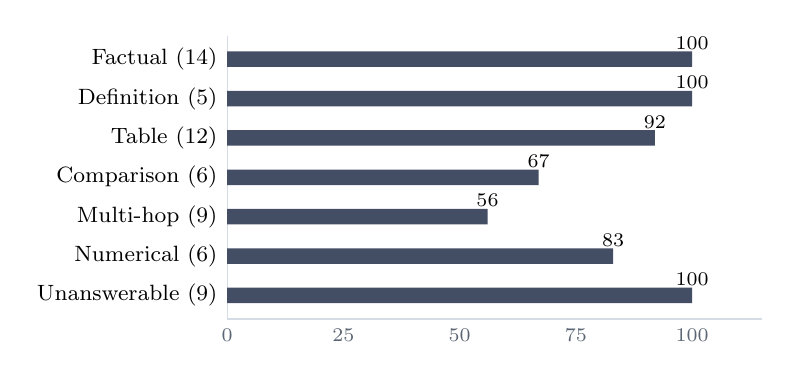
\begin{tikzpicture}
\begin{axis}[
    xbar, scale only axis, width=0.56\linewidth, height=36mm, bar width=5.6pt,
    xmin=0, xmax=115, xtick={0,25,50,75,100}, axis x line*=bottom, axis y line*=left,
    symbolic y coords={fact,def,table,comp,multi,num,unans},
    ytick=data, y dir=reverse,
    yticklabels={Factual (14), Definition (5), Table (12), Comparison (6), Multi-hop (9), Numerical (6), Unanswerable (9)},
    yticklabel style={font=\fontsize{7.6}{9}\selectfont},
    xticklabel style={font=\fontsize{7.5}{9}\selectfont,text=muted},
    nodes near coords, nodes near coords style={font=\fontsize{7.4}{9}\selectfont},
    point meta=explicit symbolic, enlarge y limits=0.1,
    axis line style={draw=rule}, major tick length=0pt]
  \addplot[fill=navy!80,draw=none] coordinates {(100,fact)[100] (100,def)[100] (92,table)[92] (67,comp)[67] (56,multi)[56] (83,num)[83] (100,unans)[100]};
\end{axis}
\end{tikzpicture}\par
\note{Percent correct, English dev set, current default. Multi-hop (5/9) is the weakest category.}
\end{minipage}

\vspace{3pt}
\textbf{How far the verifier can be trusted.} In run 6, 37 of the 40 answers the verifier marked supported were correct, and 7 of the 12 it marked unsupported were correct.
A ``verified'' label is a strong signal; an ``unsupported'' label is a weak one, which is why an unsupported answer triggers another round instead of being discarded.

% =====================================================================
\section{Many languages and scanned pages}
BGE-M3 places 100+ languages in one vector space and the reranker is multilingual, so a Hindi question can find an English passage. BM25 uses a Unicode tokenizer that keeps
Indic vowel signs inside words (a plain \texttt{\textbackslash w+} splits ``\textit{nirman}'' at every vowel sign). When the question's script differs from the document's, or the question is Hinglish,
one LLM call translates it into the document's language. The answer is written in the question's language and script, or in the one the user picks, and ``not found'' is written in about 30 languages.

\begin{minipage}[t]{0.47\textwidth}
\renewcommand{\arraystretch}{1.2}
{\fontsize{8.4}{10.2}\selectfont
\begin{tabularx}{\linewidth}{@{}X r@{}}
\toprule
Question slice (dev set, run 8) & \textbf{Correct} \\ \midrule
Hindi questions (incl.\ scanned pages) & 8/8 \\
Hinglish questions & 3/3 \\
Marathi questions & 3/3 \\
English questions about Hindi/Marathi documents & 3/4 \\
Unanswerable, correctly refused & 2/2 \\ \midrule
\textbf{All answerable} & \textbf{17/18 (94.4\%)} \\
\bottomrule
\end{tabularx}}
\note{20 questions over a Hindi article, a Marathi article, a scanned (image-only) Hindi document, and the English paper asked in Hindi and Hinglish.
Across runs of the same code the score was 16/18 or 17/18 (88.9--94.4\%); in run 6 the question that changed was the scanned Hindi one.
One answerable multilingual question was refused (1/18 false refusals).}
\end{minipage}\hfill
\begin{minipage}[t]{0.49\textwidth}
\vspace{0pt}
\begin{tcolorbox}[enhanced,colback=white,colframe=rule,boxrule=0.6pt,arc=3pt,left=0pt,right=0pt,top=0pt,bottom=0pt]
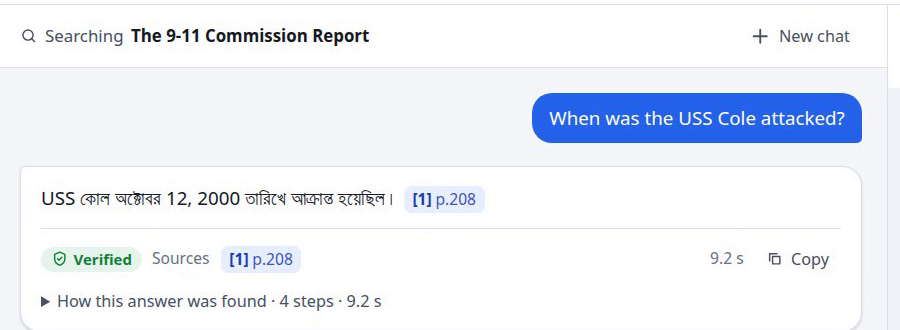
\includegraphics[width=\linewidth]{answer_lang.png}
\end{tcolorbox}
\note{An English question about the 9/11 Report with Bengali picked in the app's Answer-in menu, on a free Colab T4: ``the USS Cole was attacked on October 12, 2000'', citing page 208, verified.}
\end{minipage}

\vspace{4pt}
\textbf{22 languages (run 11).} A second set asks what users actually ask: 22 Wikipedia articles, one per language
(Hindi, Marathi, Sanskrit, Nepali, Bhojpuri, Awadhi, Maithili, Urdu, Bengali, Telugu, Tamil, Kannada, Malayalam, Gujarati, Punjabi,
Odia, English, French, Arabic, Chinese, Japanese, Russian), 14 scanned copies and 122 questions in 24 question languages, on a Kaggle
T4 x2. The system names the answer language from the question (script, then short word lists inside shared scripts), follows
``answer in Urdu'' requests and the app's Answer-in menu, writes and checks the answer in the book's language and then translates it,
tokenizes every script for keyword search, translates the question into each document script of a mixed library, keeps a passage
slot for a second matching book, picks OCR packs from Tesseract's script detection, and names the book of each citation.

\begin{minipage}[t]{0.56\textwidth}
\renewcommand{\arraystretch}{1.15}
{\fontsize{8.2}{10}\selectfont
\begin{tabularx}{\linewidth}{@{}X r@{}}
\toprule
Kind of question (dev set) & \textbf{Correct} \\ \midrule
In the document's language & 21/21 \\
English, about a non-English document & 16/20 \\
Another non-English language (Telugu on Sanskrit, ...) & 12/21 \\
``Answer in X'' request: correct / in that language & 7/8 / 7/8 \\
All 22 books searched at once: correct / right book & 19/21 / 21/21 \\
Two books in different languages: correct / both cited & 1/6 / 3/6 \\
Scanned copy (OCR) & 9/14 \\
Not in the document, refused & 9/11 \\ \midrule
\textbf{All answerable} & \textbf{85/111} \\
Answer in the right script (all 122) & \textbf{117/122} \\
\bottomrule
\end{tabularx}}
\end{minipage}\hfill
\begin{minipage}[t]{0.41\textwidth}
\vspace{0pt}
\note{Two sealed held-out sets, each run once: ten documents (Hindi, Marathi, Nepali, Awadhi, Maithili, Bengali, Kannada, Malayalam,
Odia, Japanese, four scanned) \textbf{33/44} correct, 47/48 in the right script; six documents (Sanskrit, Bhojpuri, Urdu, Telugu,
Tamil, French) \textbf{18/20}. English 45/52 and Hindi/Marathi 17/18 with the multi-language code (run 10). Weakest: a question in a
different non-English language from the book (12/21) and two-book questions (1/6), both limited by the 7B model: on the same
questions Gemma-3-12B scored 101/111 (19/21, 5/6) but refused only 6/11 unanswerable ones.}
\end{minipage}

% =====================================================================
\section{Local AI models used, and how they were chosen}
\renewcommand{\arraystretch}{1.18}
{\fontsize{8.4}{10.2}\selectfont
\begin{tabularx}{\textwidth}{@{}>{\raggedright\arraybackslash\bfseries}p{44mm} >{\raggedright\arraybackslash}X >{\raggedright\arraybackslash}p{42mm}@{}}
\toprule
\color{navy}Model (all open weights, run locally) & \color{navy}\textbf{Role} & \color{navy}\textbf{Size on the T4} \\ \midrule
Qwen2.5-7B-Instruct, 4-bit (Q4\_K\_M), Ollama, 8k context & Answers, follow-up rewriting, translation, sub-question planning, evidence grading, claim verification, calculator operands & 4.7 GB download; about 5.5--6 GB GPU memory with its cache \\
BAAI/bge-m3 (fp16) & Dense embeddings for meaning search, 100+ languages & about 1.1 GB \\
BAAI/bge-reranker-v2-m3 (fp16) & Cross-encoder reranker, multilingual & about 1.1 GB \\
BM25 (built in, Unicode-aware) & Keyword search, fused with BGE-M3 by reciprocal rank fusion & CPU, sparse matrix on disk \\
Tesseract OCR (pack chosen from each page's script) & Text from scanned pages & CPU \\
PyMuPDF layout / table model (ONNX) & Table detection; optionally on the GPU (1.89$\times$ faster, same output) & CPU or GPU \\
\bottomrule
\end{tabularx}}

\subsection{Choosing the answer model (run 8, dev sets only)}
The same pipeline was run five times on one T4, changing only the answer model: same retriever, reranker, prompts and default agent.
\renewcommand{\arraystretch}{1.2}
{\fontsize{8.3}{10}\selectfont
\begin{tabularx}{\textwidth}{@{}>{\raggedright\arraybackslash}X r r r r r r@{}}
\toprule
Answer model (4-bit) & \shortstack[r]{\textbf{English}\\\textbf{correct}} & \shortstack[r]{\textbf{Unanswerable}\\\textbf{refused}} & \shortstack[r]{\textbf{False refusals}\\\textbf{EN / ML}} & \shortstack[r]{\textbf{Latency}\\\textbf{p50 / p95}} & \shortstack[r]{\textbf{Multilingual}\\\textbf{correct}} & \shortstack[r]{\textbf{Peak GPU}\\\textbf{memory}} \\ \midrule
\textbf{Qwen2.5-7B-Instruct (chosen)} & \textbf{44/52} & \textbf{9/9} & \textbf{0} / 1 & \textbf{6.9 / 29.9 s} & \textbf{17/18} & 9,345 MiB \\
Llama-3.1-8B & 44/52 & 6/9 & 0 / 0 & 15.0 / 36.0 s & 17/18 & 10,103 MiB \\
Gemma-2-9B & 44/52 & 9/9 & 1 / 0 & 10.7 / 33.5 s & 17/18 & 12,045 MiB \\
Mistral-7B-Instruct & 39/52 & 9/9 & 3 / 2 & 9.8 / 28.6 s & 12/18 & 9,799 MiB \\
Qwen2.5-3B-Instruct & 29/52 & 8/9 & 5 / 2 & 5.3 / 14.3 s & 11/18 & 6,731 MiB \\
\bottomrule
\end{tabularx}}
\note{English: 52 answerable + 9 unanswerable questions; multilingual: 18 + 2. Peak GPU memory includes BGE-M3 and the reranker.
Qwen2.5-7B, Llama-3.1-8B and Gemma-2-9B tie on English accuracy. Qwen is kept because it refuses every unanswerable question in both sets (Llama answered 3 of the 9 English ones,
Gemma 1 of the 2 multilingual ones), has no false refusals in English, uses the least memory of the three and is the fastest. Gemma's citations were more precise (0.882 vs 0.817).
The prompts were developed with Qwen, which may favour it, and one question is 1.9 points, so differences of one to three questions are within noise.}

\textbf{Other alternatives measured and rejected.} Retrieval: MiniLM, bge-base-en, BM25 alone, English hybrid and BGE-M3 dense alone (chart above).
Reranker: none, bge-reranker-base (English) and v2-m3; v2-m3 keeps English quality and lifts multilingual recall@5 from 0.94 to 1.00. OCR: PyMuPDF's built-in OCR vs Tesseract (Hindi word recall 0.70 vs 0.99).
Table detection: a faster line-only detector invented tables in academic papers, so it stays off. Agent: single pass, always-on loop and adaptive; the always-on loop was worse than a single pass.

% =====================================================================
\section{Evaluation}
\textbf{Dev set (used during development).} English: 61 questions over three public PDFs, an ACL 2025 paper (17 pages, two columns), a U.S.\ BEA GDP release
(28 pages, 18 whitespace-aligned tables) and NIST AI 600-1 (64 pages), in seven categories including 9 the documents cannot answer. A validator checks that every
required fact appears on its cited page; a correct answer must contain every required fact and must not refuse. Multilingual: the 20 Hindi/Marathi questions and the 122-question, 22-language set of Section 5 (with a sealed 20-question held-out set).
\textbf{Held-out sets.} Questions written independently of the system by authors who read only the official sources, each document used exactly once and never re-run.

\renewcommand{\arraystretch}{1.2}
{\fontsize{8.4}{10.2}\selectfont
\begin{tabularx}{\textwidth}{@{}>{\raggedright\arraybackslash}X r r r >{\raggedright\arraybackslash}p{48mm}@{}}
\toprule
Set & \textbf{Pages} & \shortstack[r]{\textbf{Answerable}\\\textbf{correct}} & \shortstack[r]{\textbf{Unanswerable}\\\textbf{refused}} & \textbf{Notes} \\ \midrule
English dev set (runs 6 and 8) & 17--64 & \textbf{44/52} & 9/9 & 95\% interval 73.1--94.2\%; recall@5 94.2\% \\
\quad same questions, \textbf{no documents} (run 7) & -- & 1/52 & 9/9 & 46 of 52 declined; the one hit is a definition \\
Multilingual dev set (run 8) & -- & 17/18 & 2/2 & Hindi, Hinglish, Marathi, scanned Hindi \\ \midrule
\textbf{Held out:} GAO Cost Estimating Guide (run 7) & 476 & \textbf{15/18} & 2/4 & recall@5 1.000, citation precision 0.792, p50 5.4 s \\
\textbf{Held out:} US Code Title 21 (run 3) & -- & \textbf{19/25} & 4/5 & recall@5 0.917; questions naming a section 8/9 \\
\textbf{Held out:} CAG Hindi GST audit report (run 3) & 190 & \textbf{9/14} & 2/4 & answers only; Hindi 6/7, Hinglish 2/3, English 1/4 \\ \midrule
Real documents, 46 independent questions (not held out) & 585--4,211 & 30/37 & 6/9 & second run; three fixes were informed by the first \\
\bottomrule
\end{tabularx}}
\note{The GAO, Title 21 and Hindi audit sets were measured with the current answer path; the GAO run includes the number fixes. The real-document set (9/11 Report, Statistical Abstract,
US Code Title 26) was run twice and three fixes were designed from its first-run failures, so it is reported apart from the held-out sets. The CAG set's unanswerable questions were checked against the executive summary only.}

\textbf{Do the number fixes carry over?} They were tuned on the English dev set, so run 7 compared the old and new defaults on the synthetic 100- and 250-page documents (same session):
27/36 $\to$ 26/36 and 26/36 $\to$ 26/36. Numeric and table-cell questions were identical; the one difference is a section-scoped question that only the old default answered.
Outside the dev set the fixes showed no measurable gain or loss.

% =====================================================================
\section{Scale and robustness}
A fictional statistical compendium was generated at six sizes (ruled tables on 58\% of pages, two-column pages, footnotes, about 1.5\% scanned pages)
with 40 independently written questions per size, each fact planted at a known page. \textbf{This corpus shows how the system scales,
not how accurate it is on real documents:} its prose is template text, and the same questions are used at every size so that sizes can be compared.

\renewcommand{\arraystretch}{1.18}
{\fontsize{8.4}{10.2}\selectfont
\begin{tabularx}{\textwidth}{@{}*{7}{>{\raggedleft\arraybackslash}X}@{}}
\toprule
\textbf{Pages} & \textbf{Ingest (GPU tables)} & \textbf{Ingest (CPU)} & \textbf{Recall@5} & \textbf{Accuracy} & \textbf{Answer p50} & \textbf{Index on disk} \\ \midrule
100 & 30 s & 55 s & 0.972 & 0.750 & 6.3 s & 2 MB \\
250 & 58 s & 93 s & 0.972 & 0.722 & 6.3 s & 5 MB \\
1,000 & 3.8 min & 5.7 min & 0.944 & 0.722 & 6.1 s & 19 MB \\
2,500 & 9.3 min & 14.7 min & 0.944 & 0.694 & 6.8 s & 47 MB \\
5,000 & 18.2 min & 31.4 min & 0.917 & 0.750 & 6.3 s & 94 MB \\
10,000 & 36.9 min & 71.3 min & 0.889 & 0.722 & 6.0 s & 189 MB \\
\bottomrule
\end{tabularx}}
\note{Kaggle T4, run 4, 2 parse workers (the free-Colab CPU count). CPU column: an earlier run, with identical recall and accuracy at every size.
Accuracy is on the 36 answerable questions per size. Peak RAM 5.6--9.4 GB. Retrieval GPU memory stayed at 2.4 GB at every size.}

\vspace{2pt}
\begin{minipage}[t]{0.52\textwidth}
\textbf{Real long documents} \enspace {\color{muted}\fontsize{8}{10}\selectfont (Kaggle T4)}\par\vspace{2pt}
\renewcommand{\arraystretch}{1.18}
{\fontsize{8.2}{10}\selectfont
\begin{tabularx}{\linewidth}{@{}X r r r r@{}}
\toprule
 & \textbf{Pages} & \textbf{Ingest} & \shortstack[r]{\textbf{Answerable}\\\textbf{correct}} & \shortstack[r]{\textbf{Unanswerable}\\\textbf{refused}} \\ \midrule
9/11 Report & 585 & 46 s & \textbf{12/12} & 1/3 \\
Stat. Abstract & 940 & 15.7 min & \textbf{11/13} & 3/3 \\
US Code T26 & 4,211 & 11.7 min & \textbf{7/12} & 2/3 \\
\midrule
\textbf{Total} & & & \textbf{30/37} & 6/9 \\
\bottomrule
\end{tabularx}}
\note{GPU table detection, one document at a time. This set was used twice, so it is not held out. On US Code Title 26, recording each chunk's section number finds 1,877 sections (355 without it), page recall@5 0.92 (0.75).}
\end{minipage}\hfill
\begin{minipage}[t]{0.44\textwidth}
\fontsize{8.7}{10.6}\selectfont
\textbf{Recovery.} \enspace At every size, a parse worker was killed on one page and the job was cancelled half-way, then restarted.
Each time the crash cost exactly that one page, the job resumed from its checkpoint, and the index matched a clean run. At 10,000 pages the interrupted job took
4,338\,s against 4,279\,s clean (+1.4\%).\par\vspace{3pt}
\textbf{Several users.} \enspace The real web server, two answers at a time, on the 1,000-page document with 1, 2, 4 and 8 users (3 questions each): 0 failed requests of 45.
Throughput saturates at about 10.5 answers per minute; median latency rises from 12.8\,s (1 user) to 44.6\,s (8 users) as users wait in a visible queue.
First words of an answer appear after 0.47\,s (median, 1 user) and 0.70\,s (2 users).\par\vspace{3pt}
\textbf{Free-runtime memory.} \enspace Host RAM, not GPU memory, was the real limit: the Ollama runner grew by about 100\,MB per request until Colab killed the session.
Memory-mapped weights, one request slot, retries and a watchdog that restarts the runner fixed it; in the final notebook run the watchdog restarted it 5 times and no question failed.
\end{minipage}

% =====================================================================
\section{The web app and security}
The web app (FastAPI and an offline single-page frontend) puts the pipeline behind a document library:
\begin{itemize}
  \item \textbf{Library.} Uploads stream to disk with a PDF check and a size limit; a background queue shows live progress; documents left mid-way when the server stopped resume from their checkpoint at start-up.
        Several documents can be ticked and asked together; deleting a document removes its file, parsed pages and index.
  \item \textbf{Answers.} Text streams word by word, labelled as an unchecked draft until the checked, cited answer replaces it. Each citation opens the page rendered by PyMuPDF with the cited passage highlighted,
        and a trace shows every agent step.
  \item \textbf{Several users.} At most two answers run at once (configurable); others wait in a first-come queue and see their place.
  \item \textbf{Access control.} An optional access token (Bearer header or HttpOnly session cookie), one upload per client IP at a time and an optional daily upload quota.
        Every \texttt{/api} route except the health check needs the token when it is set.
  \item \textbf{Honest messages.} An audit of 25 user-visible messages fixed 12 that could mislead, for example ``verified'' shown before the check had finished, or an over-quota upload shown as ``connection closed''.
        An independent code review of the web-app and scale changes found 10 issues; 9 were fixed with regression tests (races in the partial index, quota bypasses, event order).
  \item \textbf{Tests.} 879 offline unit tests (models faked) and lint pass; CI runs them on Python 3.10 and 3.12.
\end{itemize}

% =====================================================================
\section{Deployment and requirements}
\begin{itemize}
  \item \textbf{GPU.} One NVIDIA GPU with 16 GB, tested on a Tesla T4 (free Colab and Kaggle). All three models loaded use 8.9 of 15 GB.
  \item \textbf{Host RAM.} The free Colab T4's 12.7 GB is enough; the peak was 9.4 GB during GPU table detection on the 10,000-page PDF.
  \item \textbf{Downloads.} One-time model download: about 4.7 GB for Qwen2.5-7B and about 4.5 GB for BGE-M3 and the reranker. No internet is needed afterwards.
  \item \textbf{Notebook.} \texttt{notebooks/Local\_Agentic\_RAG.ipynb} ran top to bottom on a T4 in 32.7 min with no errors, every benchmark included, and on a fresh free Colab T4.
  \item \textbf{Docker.} \texttt{docker compose up -{}-build} for a GPU machine. The image was built and an install smoke test passed with the real model on a CPU host;
        GPU inside Docker was not tested, because the T4 notebooks cannot run Docker. The CPU-only compose file works for light use: a one-page PDF took 40\,s from upload to a cited answer on a 16-core laptop CPU.
\end{itemize}

% =====================================================================
\section{Limitations}
\begin{itemize}
  \item \textbf{Multi-hop questions} that combine facts from several pages are the weakest category (5/9 on the English dev set).
  \item \textbf{Questions that presuppose something absent} (an act passed after the report) are sometimes answered from the nearest passage:
        6 of 9 unanswerable real-document questions were refused, and 2 of 4 on both the GAO and Hindi audit held-out sets. A stricter refusal rule raised false refusals from 3.8\% to 21.2\%, so it was not kept.
  \item \textbf{The number fixes} raised numerical questions to 5/6 on the English dev set they were tuned on, but showed no measurable gain on synthetic documents they were not tuned on (run 7).
  \item \textbf{Multilingual false refusal.} Qwen2.5-7B refused 1 of the 18 answerable multilingual questions; Llama-3.1-8B and Gemma-2-9B refused none (run 8).
  \item \textbf{Small benchmarks.} 61 English and 20 multilingual dev questions from one annotator; held-out sets of 18, 25 and 14 answerable questions. Grading matches required facts and can miss a paraphrase.
        95\% intervals are about $\pm$10--12 points. The real documents are four US federal PDFs and one Indian audit report.
  \item \textbf{Ingestion of table-heavy PDFs is slow on 2 CPUs:} 2.3 to 2.9 pages/s, so 10,000 pages take about 71 min (36.9 min with the opt-in GPU table detection).
  \item \textbf{Document titles from PDF metadata.} The 9/11 Report's metadata title is a print-job name (``201-635.job''), and the library shows it; the title guesser does not yet treat it as junk.
  \item \textbf{Coverage.} OCR was measured on one 2-page Hindi scan; charts and figures are not interpreted; Hindi and Marathi are not told apart by script detection.
  \item \textbf{Shared use.} The access token has no rate limit on guesses, and users behind one proxy share one upload slot. GPU inside Docker is untested.
\end{itemize}

\section{Future work}
Cell-level table retrieval and a better multi-hop strategy; a larger model such as Qwen2.5-14B for number extraction only (whether it fits beside the other models is not yet measured);
junk-title detection for PDF metadata; the section fix checked on more legal codes; a larger, multi-annotator benchmark with Hindi and Marathi long documents; rate limiting before any use
beyond one trusted group.

% =====================================================================
\section{Reproducibility}
Every number in this report was read from a run on a T4. The files \texttt{docs/RESULTS.md}, \texttt{docs/SCALE.md} and \texttt{docs/STATUS.md} record each one with its run and code snapshot.
The GPU runs were Kaggle notebooks (T4) and free Colab sessions (T4):\par
\renewcommand{\arraystretch}{1.15}
{\fontsize{8.3}{10}\selectfont
\begin{tabularx}{\textwidth}{@{}p{22mm} >{\raggedright\arraybackslash}X@{}}
\toprule
\textbf{Runs} & \textbf{What was run} \\ \midrule
Colab runs & Project notebook top to bottom on a fresh Colab T4; end-to-end answer and multilingual benchmarks \\
Validation, scale v1--v4, run 1 & Notebook top to bottom on a Kaggle T4 (32.7 min); scale benchmark 100--10,000 pages with recovery and load test; real long documents; streaming and asking while processing \\
Runs 2--4 & Section numbers and the layout model on the GPU (run 2); run 3, the final run (real documents, held-out Title 21 and Hindi audit, regression); run 4 (six scale tiers) \\
Runs 5 and 6 & Number fixes, one flag at a time, and the previous vs the current default in one session \\
Runs 7 and 8 & No-document control, GAO held-out set, number-fix carry-over (run 7); five answer models (run 8); demo recording on a free Colab T4 \\
Runs 9--11 & 22 languages: development set, the two sealed held-out sets, and Qwen3-8B and Gemma-3-12B on the same questions \\
\bottomrule
\end{tabularx}}

\vspace{3pt}
To reproduce (held-out sets are not re-run: each was used once):
\begin{itemize}
  \item \texttt{python benchmark/fetch\_pdfs.py}, then \texttt{python -m local\_agentic\_rag.bench retrieval}
  \item \texttt{python -m local\_agentic\_rag.bench answer -{}-llm ollama:qwen2.5:7b-instruct}
  \item long documents: \texttt{python benchmark/scale/run\_scale.py}; offline tests: \texttt{pytest -q}
\end{itemize}

\end{document}
